\documentclass{beamer}
\usepackage[utf8]{inputenc}

\usetheme{Madrid}
\usecolortheme{default}
\useinnertheme{circles}

\definecolor{Logo1}{rgb}{0.208, 0.2865, 0.373}
\definecolor{Logo2}{rgb}{0.000, 0.674, 0.863}

\setbeamercolor*{palette primary}{bg=Logo1, fg=white}
\setbeamercolor*{palette secondary}{bg=Logo2, fg=white}
\setbeamercolor*{palette tertiary}{bg=white, fg=Logo1}
\setbeamercolor*{palette quaternary}{bg=Logo1,fg=white}
\setbeamercolor{structure}{fg=Logo1} % itemize, enumerate, etc
\setbeamercolor{section in toc}{fg=Logo1} % TOC sections

%-----------------------------------------------------------
\title[]{Cloud Computing Case Study: Amazon Web Services}
\author[]{Debanjan Kola, Sauvik Dutta, Sankha Ghosh, Somnath Ganguly}

\institute[]{
  Department of Computer Science\\
  Ramakrishna Mission Vivekananda Centenary College
}
\date[]{August 2024}


%\logo{
\includegraphics[height=.5cm]{logo-footer.png}}


\AtBeginSection[]
{
  \begin{frame}
    \frametitle{Table of Contents}
    \tableofcontents[currentsection]
  \end{frame}
}
%------------------------------------------------------------


\begin{document}


\frame{\titlepage}


\begin{frame}
\frametitle{Table of Contents}
\tableofcontents
\end{frame}



\section{AWS as Platform as a Service (PaaS)}

\begin{frame}
\frametitle{What is PaaS?}
\begin{block}{Defintion}
	Platform as a Service (PaaS) is a cloud computing model that provides a platform allowing customers to develop, run, and manage applications without the complexity of building and maintaining the underlying infrastructure.
\end{block}
\end{frame}


\begin{frame}
	\frametitle{Two-column slide}
	\begin{examples}{AWS Services that belongs to PAAS}
		\begin{itemize}
			\item AWS Lambda
			\item AWS Elastic Beanstalk
		\end{itemize}
	\end{examples}		
\end{frame}

\begin{frame}
	\frametitle{AWS Lambda}
	\begin{block}{Defintion}
		AWS Lambda is a serverless computing service that lets the developers run their code in the standard runtime environment of Lambda without having to worry about server handling with zero supervision.
	\end{block}
	
	\begin{center}
	
	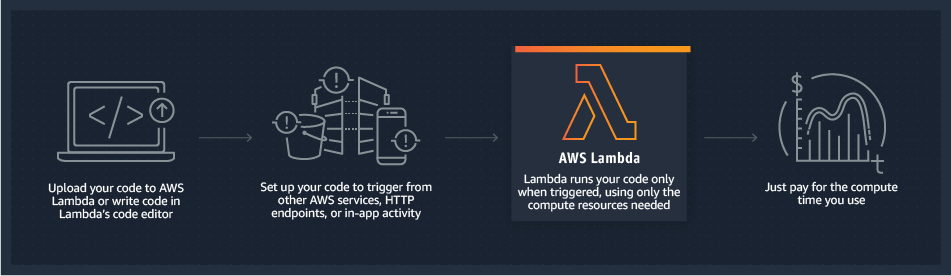
\includegraphics[scale=0.35]{product-page-diagram_Lambda-HowItWorks.68a0bcacfcf46fccf04b97f16b686ea44494303f.png}
	\end{center}
\end{frame}

\begin{frame}
	\frametitle{AWS Lambda}
	\begin{alertblock}{Important Note}
		To develop any AWS service or application, creating a Lambda function is a must.
	\end{alertblock}
	
\end{frame}

\section{Second section}


\begin{frame}
\frametitle{Sample frame title}

\end{frame}

\begin{frame}
\frametitle{Two-column slide}

\end{frame}

\begin{frame}
	\frametitle{Two-column slide}	
\end{frame}

\begin{frame}
	\frametitle{Two-column slide}	
\end{frame}


\begin{frame}
	\frametitle{Two-column slide}	
\end{frame}


\begin{frame}
	\frametitle{Two-column slide}	
\end{frame}


\begin{frame}
	\frametitle{Two-column slide}	
\end{frame}


\begin{frame}
	\frametitle{Two-column slide}	
\end{frame}


\begin{frame}
	\frametitle{Two-column slide}	
\end{frame}


\begin{frame}
	\frametitle{Two-column slide}	
\end{frame}


\begin{frame}
	\frametitle{Two-column slide}	
\end{frame}


\begin{frame}
	\frametitle{Two-column slide}	
\end{frame}


\begin{frame}
	\frametitle{Two-column slide}	
\end{frame}


\begin{frame}
	\frametitle{Two-column slide}	
\end{frame}


\begin{frame}
	\frametitle{Two-column slide}	
\end{frame}


\begin{frame}
	\frametitle{Two-column slide}	
\end{frame}


\begin{frame}
	\frametitle{Two-column slide}	
\end{frame}


\begin{frame}
	\frametitle{Two-column slide}	
\end{frame}


\begin{frame}
	\frametitle{Two-column slide}	
\end{frame}


\begin{frame}
	\frametitle{Two-column slide}	
\end{frame}

\begin{frame}
	\frametitle{Two-column slide}	
\end{frame}

\begin{frame}
	\frametitle{Two-column slide}	
\end{frame}

\begin{frame}
	\frametitle{Two-column slide}	
\end{frame}


\begin{frame}
	\frametitle{Two-column slide}	
\end{frame}


\begin{frame}
	\frametitle{Two-column slide}	
\end{frame}


\begin{frame}
	\frametitle{Two-column slide}	
\end{frame}

\begin{frame}
	\frametitle{Two-column slide}	
\end{frame}

\begin{frame}
	\frametitle{Two-column slide}	
\end{frame}


\begin{frame}
	\frametitle{Two-column slide}	
\end{frame}


\begin{frame}
	\frametitle{Two-column slide}	
\end{frame}


\begin{frame}
	\frametitle{Two-column slide}	
\end{frame}


\begin{frame}
	\frametitle{Two-column slide}	
\end{frame}

\begin{frame}
	\frametitle{Two-column slide}	
\end{frame}

\begin{frame}
	\frametitle{Two-column slide}	
\end{frame}


\begin{frame}
	\frametitle{Two-column slide}	
\end{frame}


\begin{frame}
	\frametitle{Two-column slide}	
\end{frame}


\begin{frame}
	\frametitle{Two-column slide}	
\end{frame}


\begin{frame}
	\frametitle{Two-column slide}	
\end{frame}

\begin{frame}
	\frametitle{Two-column slide}	
\end{frame}

\begin{frame}
	\frametitle{Two-column slide}	
\end{frame}


\begin{frame}
	\frametitle{Two-column slide}	
\end{frame}


\begin{frame}
	\frametitle{Two-column slide}	
\end{frame}


\begin{frame}
	\frametitle{Two-column slide}	
\end{frame}


\begin{frame}
	\frametitle{Two-column slide}	
\end{frame}

\begin{frame}
	\frametitle{Two-column slide}	
\end{frame}

\begin{frame}
	\frametitle{Two-column slide}	
\end{frame}


\begin{frame}
	\frametitle{Two-column slide}	
\end{frame}


\begin{frame}
	\frametitle{Two-column slide}	
\end{frame}


\begin{frame}
	\frametitle{Two-column slide}	
\end{frame}


\begin{frame}
	\frametitle{Two-column slide}	
\end{frame}

\begin{frame}
	\frametitle{Two-column slide}	
\end{frame}

\begin{frame}
	\frametitle{Two-column slide}	
\end{frame}


\begin{frame}
	\frametitle{Two-column slide}	
\end{frame}


\begin{frame}
	\frametitle{Two-column slide}	
\end{frame}


\begin{frame}
	\frametitle{Two-column slide}	
\end{frame}


\begin{frame}
	\frametitle{Two-column slide}	
\end{frame}

\begin{frame}
	\frametitle{Two-column slide}	
\end{frame}

\begin{frame}
	\frametitle{Two-column slide}	
\end{frame}



\end{document}